\documentclass[aps,prx,10pt,twocolumn,floatfix,superscriptaddress,showpacs,numerical,footinbib]{revtex4-1}

\usepackage{graphicx}
\usepackage{amsmath}
\usepackage{amssymb}
\usepackage[utf8]{inputenc}
\usepackage{hyperref}
\usepackage[pdftex]{color}

\newcommand{\sgn}[1]{\mathrm{sgn} \left( #1 \right)}
\newcommand{\e}{\mathrm{e}}
\newcommand{\im}{\mathrm{i}}
\newcommand{\di}{\mathrm{d}}
\newcommand{\ket}[1]{| #1 \rangle}
\newcommand{\bra}[1]{\langle #1 |}
%\renewcommand{\thefootnote}{\fnsymbol{footnote}}

\newcommand{\noteAG}[1]{{\color{blue} [AG: #1]}}
\newcommand{\noteFP}[1]{{\color{magenta} [FP: #1]}}
\newcommand{\noteJM}[1]{{\color{red} [JM: #1]}}
\newcommand{\noteFdJ}[1]{{\color{cyan} [FdJ: #1]}}
\newcommand{\bs}[1]{{\boldsymbol{#1}}}


\begin{document}
%
\title{Interaction driven phases in the half-filled honeycomb lattice: an infinite density matrix renormalization group study}
%
\author{Good people}
\affiliation{\mbox{Max-Planck-Institut f\"ur Physik komplexer Systeme, N\"othnitzer Str.\ 38, 01187 Dresden, Germany}}
%
\date{\today}
%
\begin{abstract}
%
This is an abstract.
%
\noteAG{There are specific commands to leave comments like this one}\noteFP{or this}\noteJM{or this}\noteFdJ{or this}
%
\end{abstract}
%
\maketitle
%

\section{Introduction}
%
Although in the last decade

Interactions and topological states~\cite{H88}.\\
%

%
Due to its singular importance and historical significance, 
the emergence of the Chern insulator state via interactions in the honeycomb lattice is an active
research area. 
%


%
In this work we revisit the controversies left unsolved by previous works using the infinite density matrix renormalzation group method (iDMRG). \\


\section{Model and Method}
%
In this work we focus on spinless electrons hoping on a honeycomb lattice with real nearest neighbor hopping $t$ interacting via nearest and next to nearest neighbor interactions 
$\left\lbrace V_{1},V_{2}\right\rbrace$ respectively. 
%
The Hamiltonian for this system can be written as
 %
\begin{eqnarray}
\nonumber
%
H&:=&-t\sum_{\left\langle i,j\right\rangle ,s,s'}(c^{\dagger}_{i,s}c_{j,s'}+h.c.)\\
%
\;&+&
V_{1}\sum_{\left\langle i,j\right\rangle ,s }n_{i,s}n_{j,\bar{s}}+
%
V_{2}\sum_{\left\langle \left\langle i,j\right\rangle \right\rangle ,s }n_{i,s}n_{j,s}\,
%
\label{eq:H}
%
\end{eqnarray}
%
here $c_{i,s}$ $(c^{\dagger}_{i,s})$  annihilates (creates) an electron at the $i$-th unit cell of the honeycomb lattice
in sublattice $s=A,B$ and $s\neq\bar{s}$. 
%
Each of the two triangular sublattices A and B is spanned by the basis vectors
$\bs{a}_{1}=\bs{\delta}_{2}-\bs{\delta}_{3}$ and 
$\bs{a}_{2}=\bs{\delta}_{3}-\bs{\delta}_{1}$ defined through the three nearest neighbors $\bs{\delta}_{1}=a(0,-1)$,  
$\bs{\delta}_{2}=a(\sqrt{3}/2,1/2)$ and $\bs{\delta}_{3}=a(-\sqrt{3}/2,+1/2)$ as shown in Fig.~\ref{fig:Defs}.\\
%

In order to find the ground state of the system in the $\left\lbrace V_{1},V_{2}\right\rbrace$ phase space
we use the infinite density matrix renormalzation group method (iDMRG). 
%
\noteAG{we might want to define the entanglement spectrum here also if we ever use it}\\
\noteAG{Define correlation length as well}
\noteAG{We might want to discuss which cylinder sizes we use and why. Namely L=6,12 include the K points while L=8,10 don't.}
%

\begin{figure}
 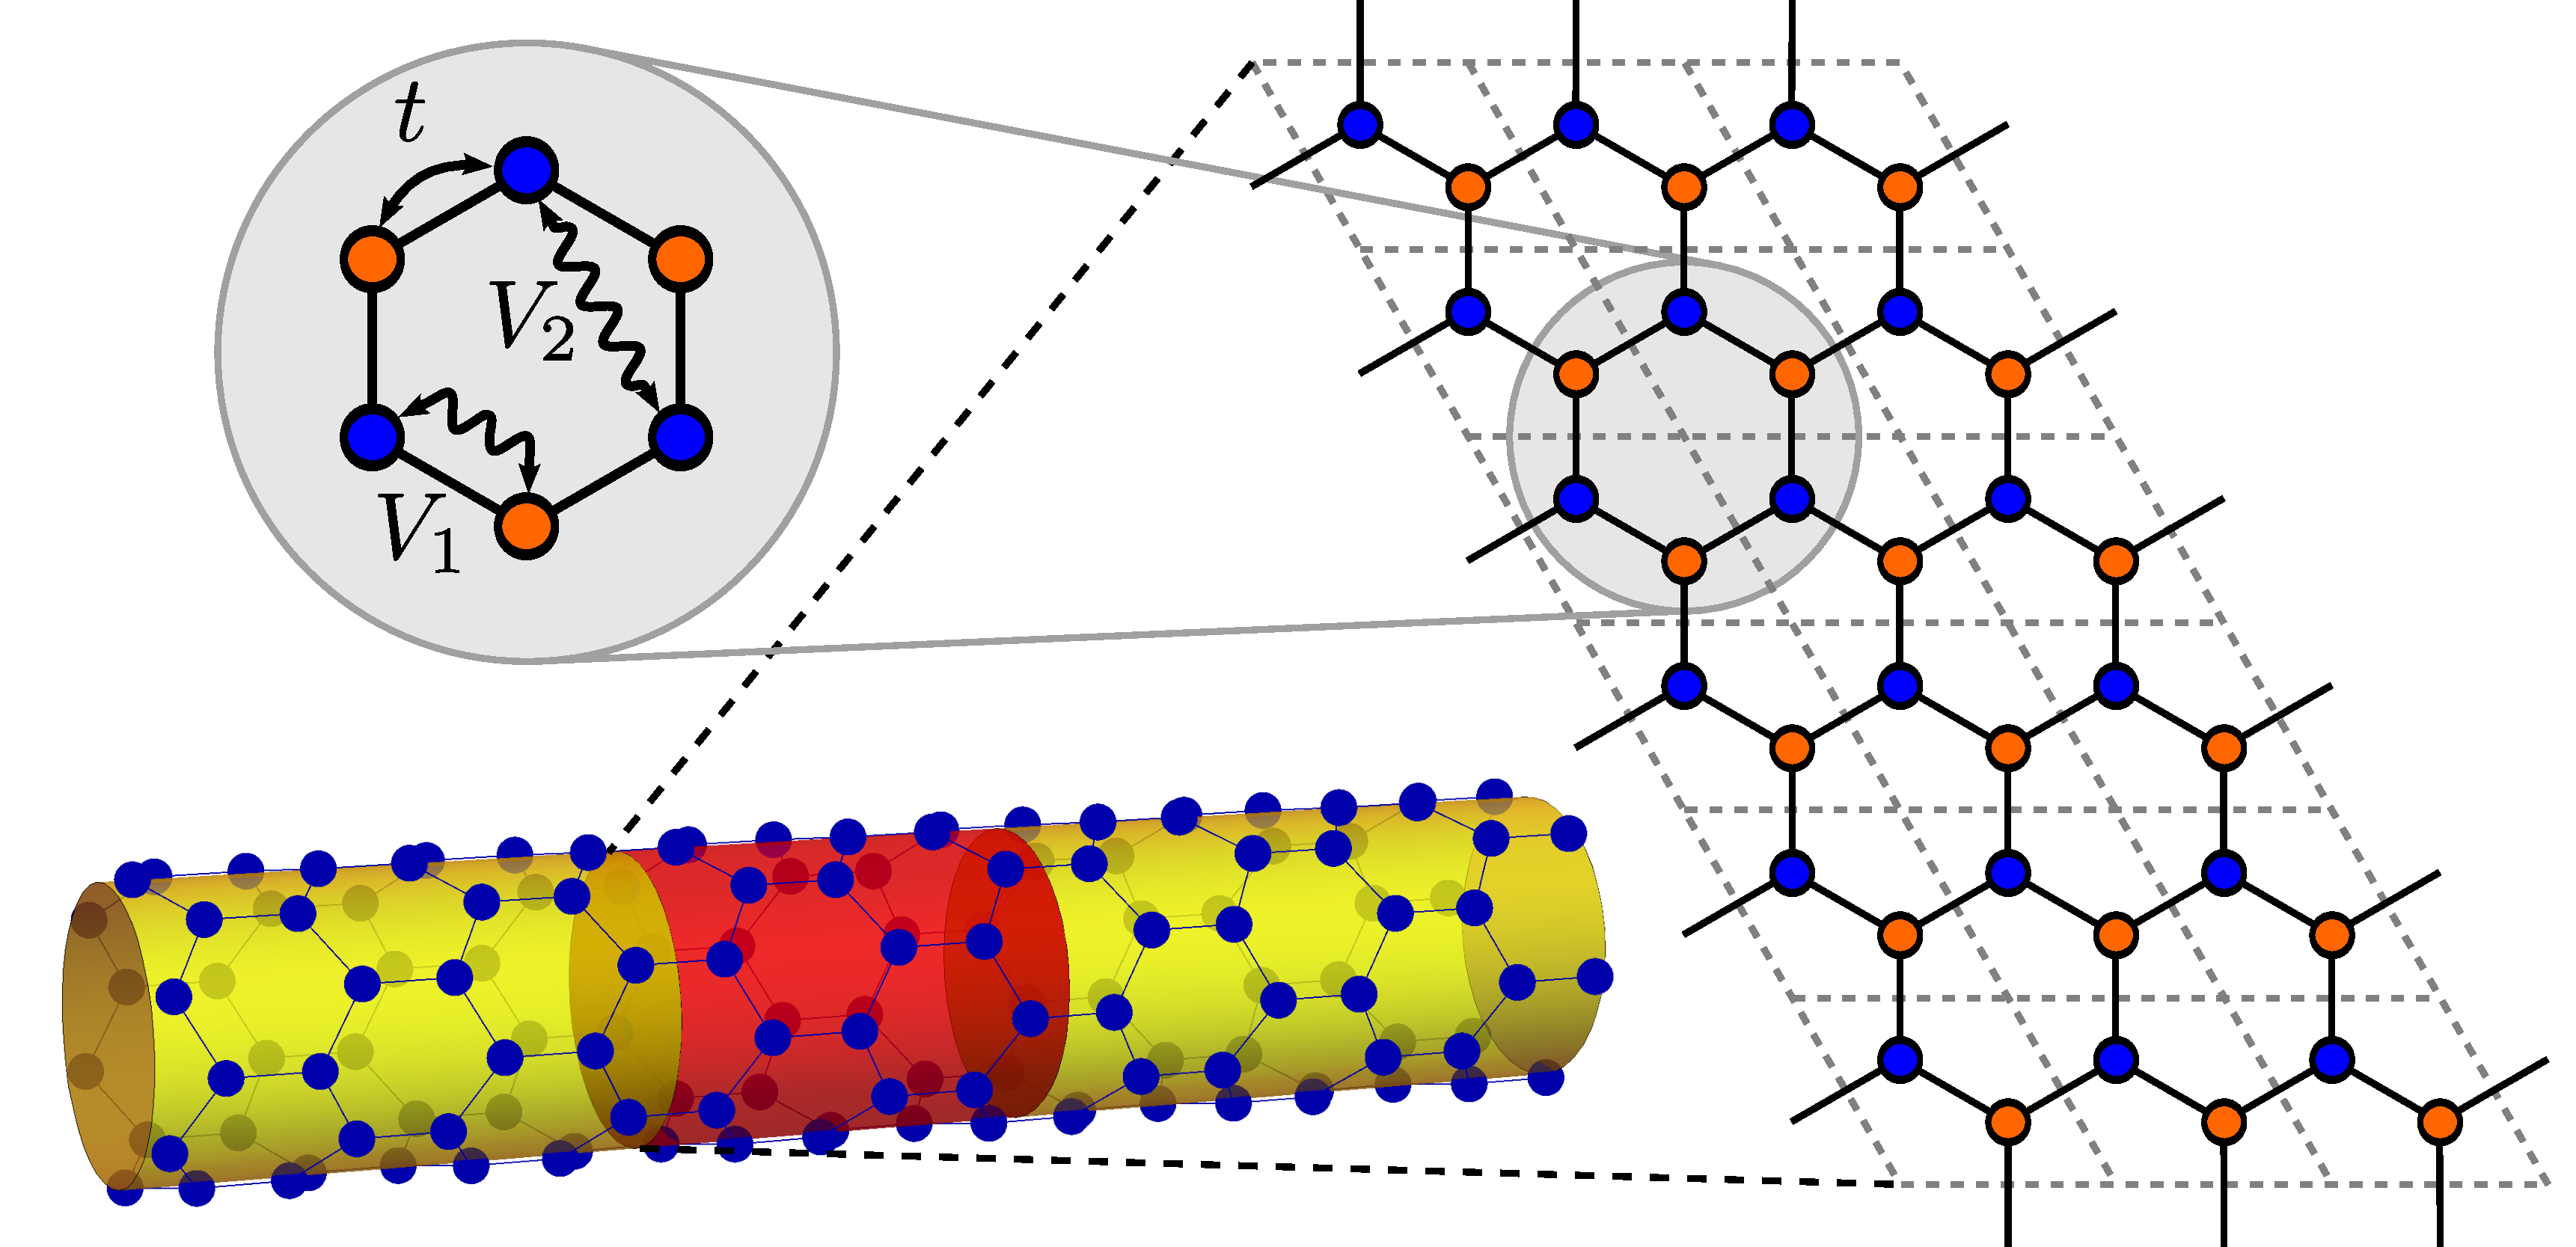
\includegraphics[scale=0.2]{pdf/unit_cell.pdf}
 \caption{Left: Hoppings and interactions of Hamiltonian \eqref{eq:H}. Right: Honeycomb lattice of $3 \times 2$ unit cells. The unit cell used for the iDMRG calculations consists of $3 \times 6$ honeycomb unit cells which yields a total circumference of 12 sites. \label{fig:Defs}}
\end{figure}
%
\begin{figure*}[tb]
 \includegraphics[scale=0.2]{Fig1.eps}
 \caption{ 
  }
  \label{fig:honeycomblattice}
\end{figure*} 
%% 
\section{Phase diagram}
%
We have used the iDMRG method presented in the previous section
to find the groundstate of the half-filled graphene lattice in the presence of 
$\left\lbrace V_{1},V_{2}\right\rbrace$ interactions.
%
Our results are summarised in the phase diagram presented in Fig.~\ref{fig:phase diagram}.
%
As a function of $\left\lbrace V_{1},V_{2}\right\rbrace$ we find six different phases and none of them correspond to the Haldane Chern insulator.
%
In what follows we describe their corresponding charge and bond ordering patterns and analyse the different phase transitions that occur between them.
%

\begin{figure}
 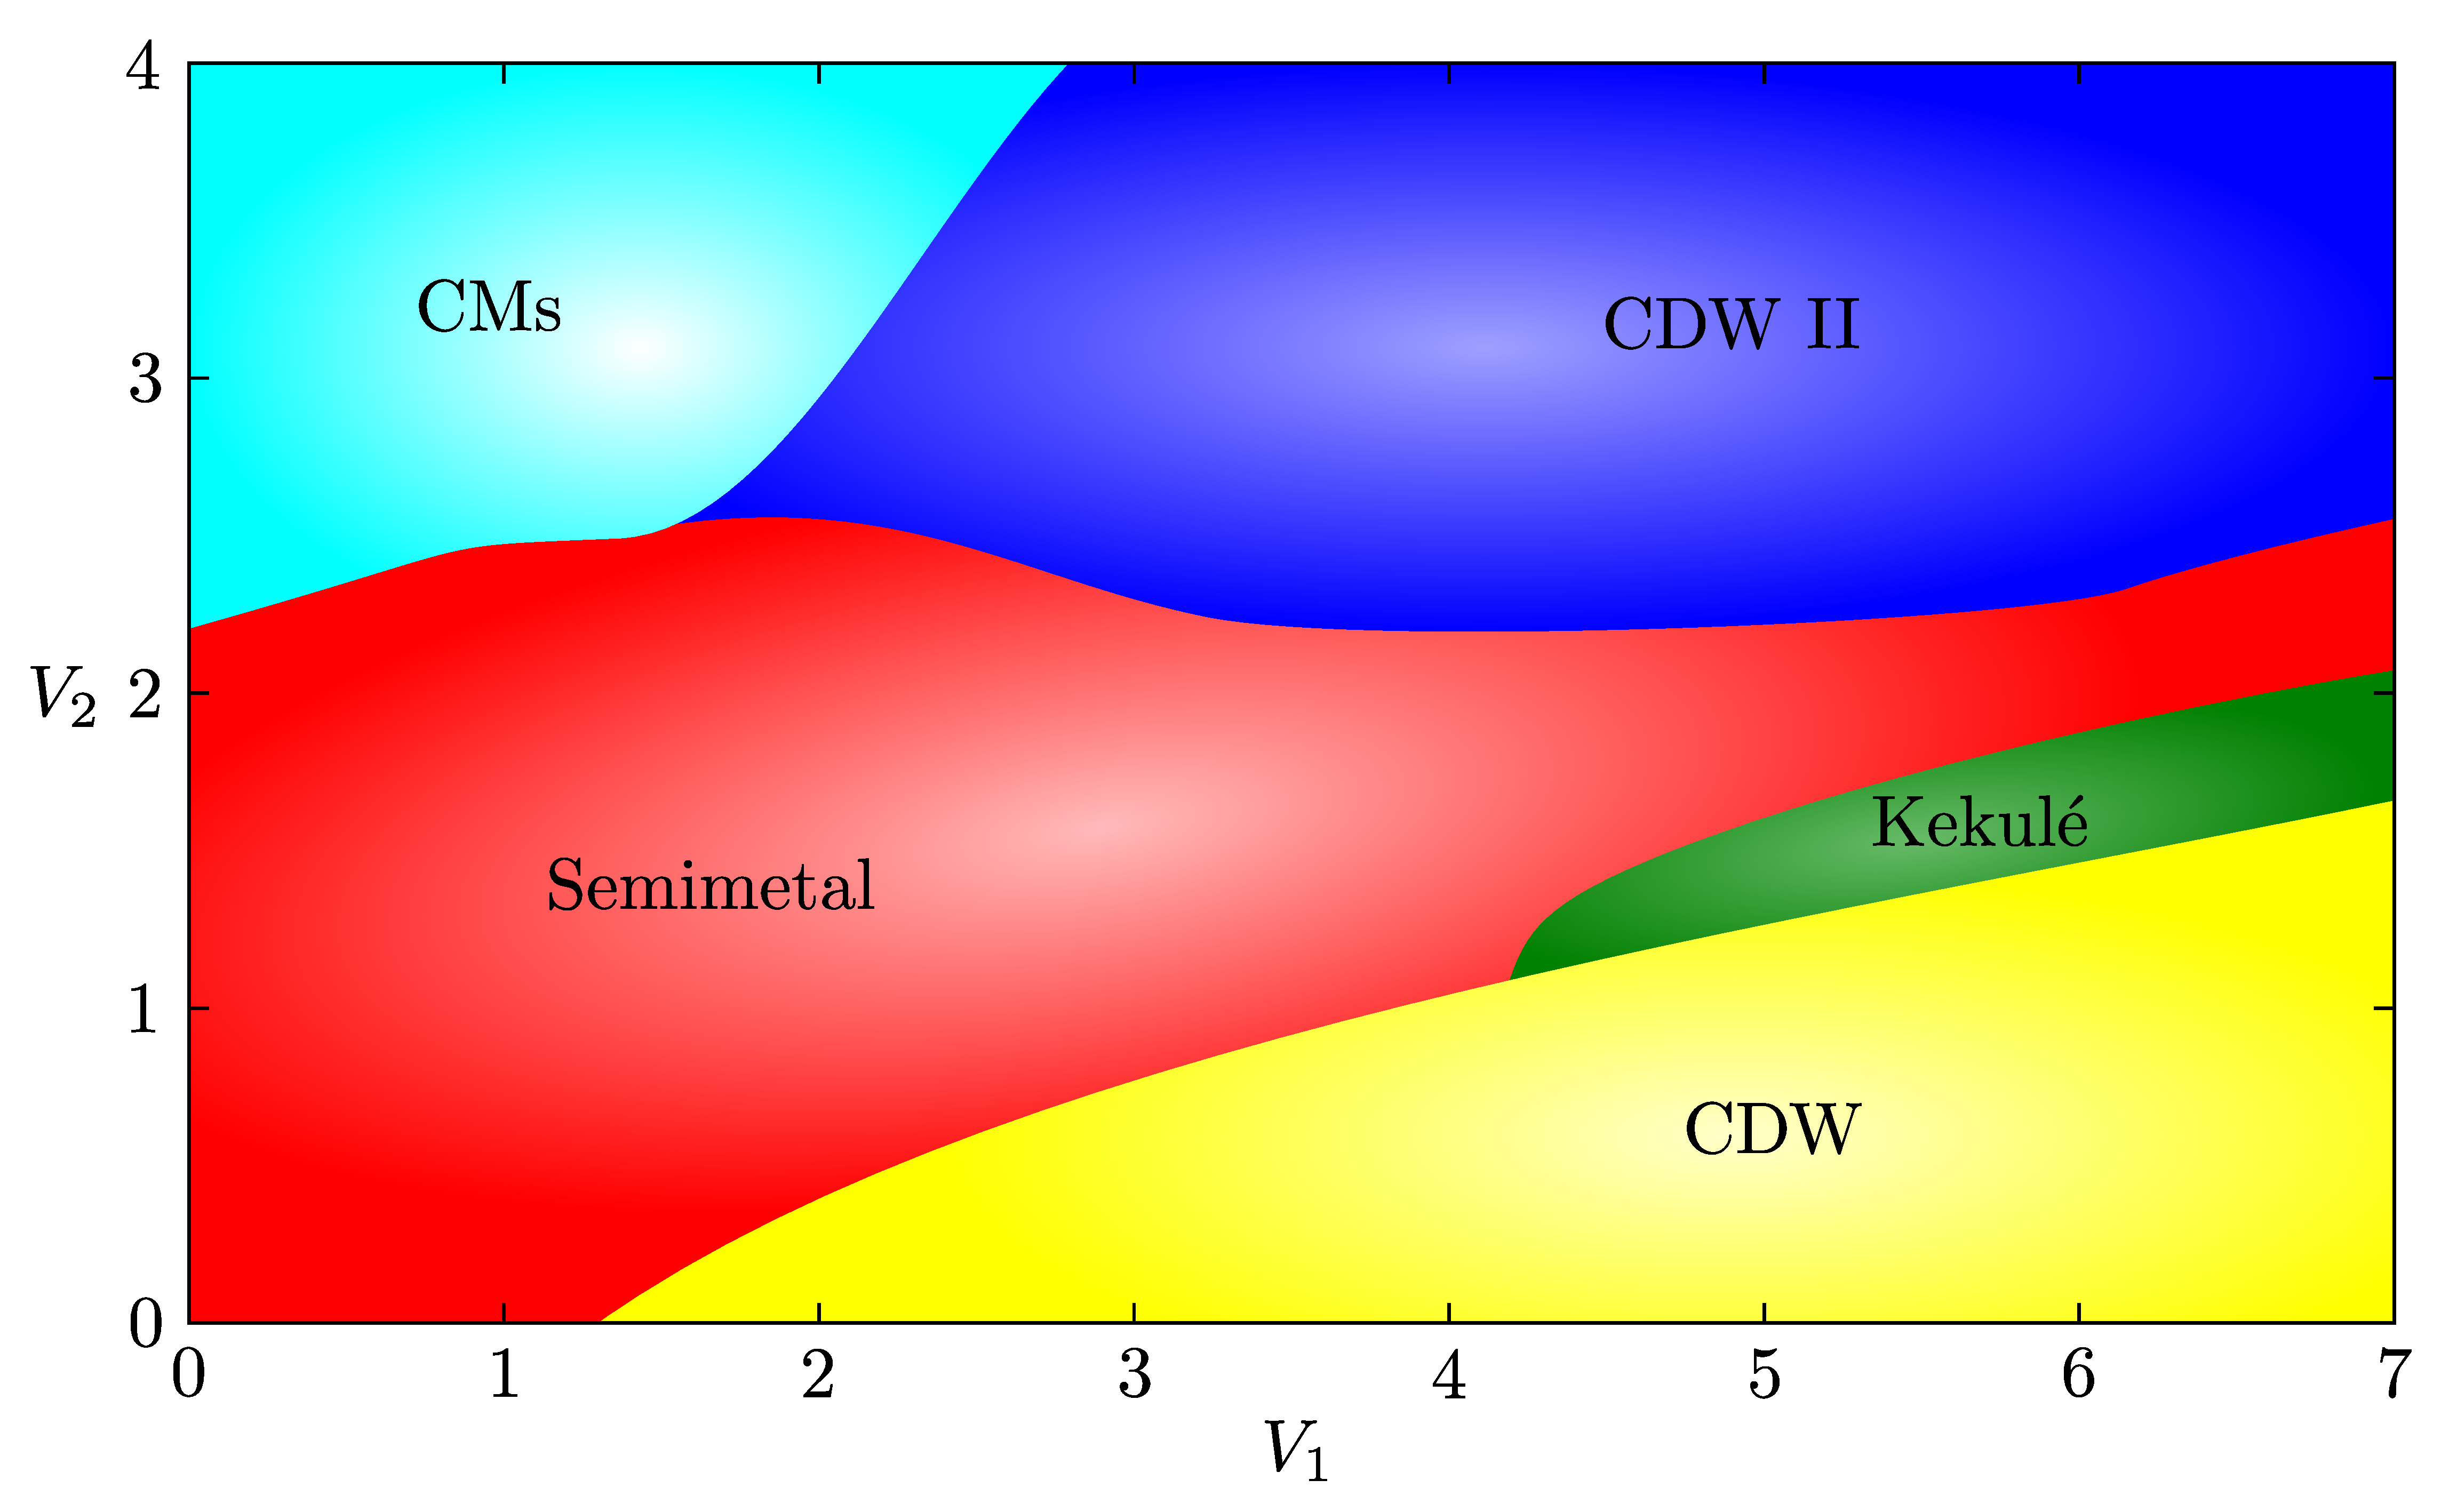
\includegraphics[width=\columnwidth]{pdf/phase_diagram.pdf}
 \caption{Phase diagram obtained with iDMRG calculations on an infinte cylinder of circumference $L=12$. \label{fig:phase diagram}}
\end{figure}

%
\subsection{Semimetal phase (SM)}
%
We start by discussing the semimetal phase, labelled SM in the phase diagram shown in Fig.~\ref{}.
%
This phase is continuously connected to the gapless non-interacting state $V_{1}=V_{2}=0$; 
it is a uniform renormalization of the hopping strength $t$ by interactions.
%
Therefore we identify this state as a single particle gapless phase that lacks both charge and bond order and is described by a low energy theory in terms of two massless Dirac fermions.
%
We note that in such low energy picture and within the renormalisation group approach the stability of the semimetal phase in the region $\left\lbrace V_{1},V_{2}\right\rbrace < t$ is expected.
%
Short range interactions are irrelevant~\cite{Shankar?} and therefore they can only drive a transition to an ordered state when they have a magnitude comparable to the nearest neighbour hopping strength $t$.
%
Accordingly we find that the semimetal is stable within this region of phase space.

Within the iDMRG algorithm we have characterised the semimetal phase in three distinct ways.
%
Firstly we compute the charge and bond ground state expectation values.
%
On the one hand, at each site the charge expectation value is defined by 
%
\begin{eqnarray}
\label{eq:charge}
n_{i,s}=\left\langle c^{\dagger}_{i,s}c_{i,s}\right\rangle,  
\end{eqnarray}
%
where $s=A,B$ is the sublattice index.
%
To numerical accuracy we find that $n_{i,A}=n_{i,B}=1/2$, indicating that this phase is not charge ordered.
%

The bond ground state expectation value on the other hand is defined as
%
\begin{eqnarray}
\label{eq:bond}
t^{s,s'}_{i,j}=\left\langle c^{\dagger}_{i,s}c_{j,s'}\right\rangle,  
\end{eqnarray}
%
For $i,j$ being nearest neighbours we find a small ($10^{-?}$ \noteAG{number needed}) asymmetry
between bonds pointing along and around the cylinder axis.
%
Such asymmetry should vanish in a perfect semimetalic phase and indeed it is severely reduced as the bond dimension $\chi$ is increased.
% 
This suggests that the explanation for the asymmetry is indeed the cylinder geometry implemented in iDMRG, that artificially differentiates bonds in its two perpendicular directions.
%

%
Moreover, we note that the semimetal phase is a critical state and thus in principle requires an infinite $\chi$ to represent the state.
%
This leads us to the second approach to characterise the semimetal phase that makes use of the its criticality.
%
For a critical phase the entanglement entropy is expected to show a logarithmic growth with the correlation length.
\noteAG{eqn needed}
%
The proportionality constant $c/3$ defines the central charge of the theory $c$. 
%
The semimetal has two Dirac cones and therefore it is expected that $c=2$. 
%
In the appendix...
\noteAG{This last paragraph can be removed if we don't need it}

%
Lastly we find that the low energy structure of the many-body 
entanglement spectrum of this phase exactly coincides with that of the parent non-interacting critical state.\\ 
%

%
We note finally that this state extends beyond 

\subsection{Charge density wave (CDW)}
%
The second state we identify is the charge density wave state, labelled CDW in the phase diagram of Fig.~\ref{}.
%
This state has a two site unit cell that is characterised by a finite order parameter
%
\begin{equation}
\label{eq:CDW}
%
M=\left\langle n_{A} \right\rangle-\left\langle n_{B}\right\rangle
%
\end{equation}
%
where $n_{A}$ and $n_{B}$ are the density of electrons in the $A$ and $B$ sublattice sites of the two site unit cell respectively.
%
We find that the magnitude of $M$ increases with $V_{1}$ and to numerical accuracy this phase has no appreciable bond order.\\
%

For large $V_{1}\gg t$ such a state is a natural instability since the energy is minimised by a charge imbalance between the two sub lattices.
%
Indeed, it has been found in a mean field approximation~\cite{Raghu,Franz,us}, exact diagnoalization~\cite{us,daghofer,herbut}, and quantum Monte Carlo simulations
\cite{QMC}.
%


\subsection{Sub-lattice charge modulated phase (CMs)}
%
For large $V_{2}\ll t$ the ground state is classically degenerate. 
%
Within mean field it was shown that as long $V_{2}>V_{1}$
the system chose a charge ordered pattern with charge modulation over different sub lattices and termed CMs phase~\cite{CMs}.
%
Such order, schematically shown in Fig.~\ref{}, has a six site unit cell, and minimises the large cost
attributed to $V_{2}$ by reversing two nearest neighbour dimers at the expense of paying the small energetic cost
determined by $V_{1}$.
%
Within in exact diagonalization two studies has shown that the CMs state survives quantum fluctuations 
but its nature was challenged in Ref.~\onlinecite{daghofer} suggesting that a pinball like state cannot be ruled out.\\

With the iDMRG method (see Fig.~\cite{s}) we find that directly above the semimetallic phase the CMs occurs with the right type of order.
%
The calculated charge pattern obtained from \eqref{eq:charge} is shown in Fig.~\cite{} panel, which resembles the expected
CMs pattern.
%
The six-site unit cell is depicted as a red hexagon for clarity. 
%
Such a state also presents bond ordering associated to the charge patterns.

% 
Moreover, we now show that the CMs state is expected from a semi-classical analysis as well.
%
For instance, for a given cluster, it is possible to find the number and energy of all the degenerate classical states, assuming $V_{2}\gg t$.
%
Within this approach, the hopping can be introduced as a perturbation $t$ to find how the degeneracy is lifted.
\noteAG{Maybe Fernando can rewrite this part better...} 


\subsection{Kekul\'{e} bond order}
%
The next phase we identify is the Kekul\'{e}
bond order.
%
Like the CMs, it has a six site unit cell depicted schematically in Fig.~\ref{}
and uniform charge order.
%
In mean field the state arises close to the $V_{1}\eqsim V_{2}$.
%
Although in exact diagonalization hints of this state are also observed,
the evidence supporting its occurrence is far from conclusive.



\subsection{Charge density wave - II}
%
All phases that we have described so far don't differ
from those predicted by mean field and exact diagonalization.
%
We have identified
%
\subsection{Charge density wave - III}
%



\section{Phase transitons}
%
A crucial advantage of the iDMRG method is that, unlike finite
size methods such as exact diagonalization it can characterize the order of phase transitions.
%
In order to unravel the character of the phase transitions between
the phases described above we now study two quantities that are sensitive
to a phase change, the entanglement entropy $S$ and the correlation length $\xi$.
%
In Fig.~\ref{}  and Fig.~\ref{} we show how these quantities change along
the horizontal and vertical cuts depicted in Fig.~\ref{fig:phase diagram} respectively.
%

\subsection{Cut A: SM--CDW-I}

The first horizontal cut, labelled A addresses the character of the phase transition between the semi-metallic
phase and the simplest charge density wave (CDW-I) by fixing $V_{2}=0$.
%
This phase transition has been previously addressed with the quantum Monte-Carlo method~\ref{papers} 
and was determined to be of second order character.
%
The transition point with divergent correlation length was determined to be at $V_{1}=$ via finite size scaling.
\noteAG{need number and polishing, Johannes?}\\
%
In Fig.~\ref{} we show the correlation length as a function of $V_{1}$ 
for different values of the bond dimension $\chi$ and cylinder with $L=12$ circumference.
%
Firstly, for $V_{1}\leq 1.5t$ we observe that the correlation length diverges as the bond
dimension of the MPS is increased.
%
This behaviour is expected for a critical state such as the semimetal phase;  
the logarithmic divergence of entanglement of a metallic state requires an MPS with $\chi\to\infty$.
%
For $V_{1}\geq 1.5t$ the correlation length drops significantly and has no longer a significant 
dependence on $\chi$.
%
This is characteristic of a gapped phase such as the charge density wave.
%
The crossover is smooth, signalling a second order phase transition, in agreement with 
quantum Monte Carlo studies.
%
With iDMRG it is however not possible to pin point the exact value of $V_{1}$ 
where the transition happens via finite size scaling due to the few cylinder sizes 
we have available \footnote{}.
%
From Fig.~\ref{} it is however possible to define a crossover region $1.4 \leq V_{1}\geq 2$,
consistent with the quantum Monte Carlo data, where the transition occurs.

\subsection{Cut B: SM--CMs}
%
A cut at $V_{1}=0.4$, labelled cut B in Fig.~\ref{fig:phasediagram}, 
probes the transition between the semimetal phase and the CMs phases.
%
In Fig.~\ref{} we present the entanglement entropy $S$ as a function of 






\begin{figure}
 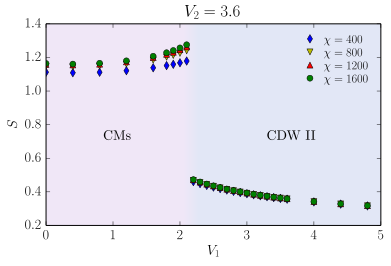
\includegraphics[width=\columnwidth]{{pdf/plot_cut_V2_3.6}.pdf}
 \caption{Entanglement entropy at $V_2=3.6$. \label{fig:cut_V2_3.6}}
\end{figure}

\begin{figure}
 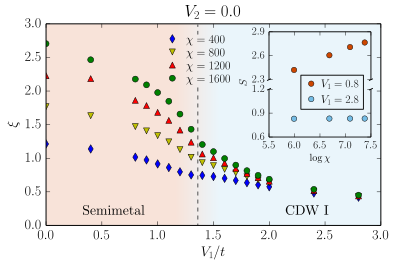
\includegraphics[width=\columnwidth]{{pdf/plot_cut_V2_0}.pdf}
 \label{fig:cut_V2_0}
 \caption{Correlation length at $V_2=0$.  \noteAG{could it be useful to show the order parameter M
 as a function of $V_{1}$ in the same plot (using the right vertical axis?, or it might be to crowded)}}
\end{figure}

\begin{figure}
 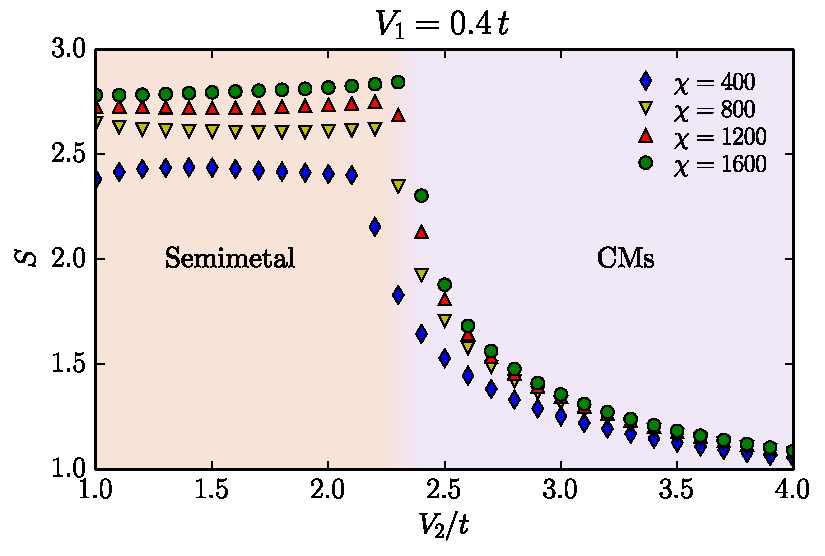
\includegraphics[width=\columnwidth]{{pdf/plot_cut_V1_0.4}.pdf}
 \caption{Entanglement entropy at $V_1=0.4$. \label{fig:cut_V1_0.4}}
\end{figure}

\begin{figure}
 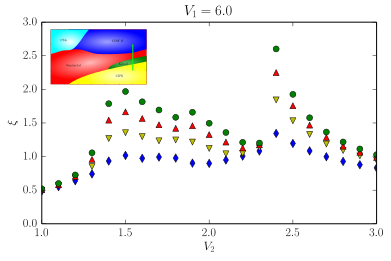
\includegraphics[width=\columnwidth]{{pdf/plot_cut_V1_6}.pdf}
 \caption{Correlation length at $V_1=6$. \label{fig:cut_V1_6}}
\end{figure}



%
\section{Discussion and Conclusions}
%
No CI phase\\
%
Two new phases not seen before\\
%
What determines if $S$ or $\xi$ gives better signatures of phase transitions. 

\section{Acknowledgements}

We thank A. Lauchli for discussions and sharing results prior to publication.

\bibliography{CI_iDMRG.bib}


\end{document}